\documentclass[11pt]{article}
\usepackage{coling2014}
\usepackage{times}
\usepackage{url}
\usepackage{latexsym}
\usepackage{graphicx}
\usepackage{amsmath}

%\setlength\titlebox{5cm}

% You can expand the titlebox if you need extra space
% to show all the authors. Please do not make the titlebox
% smaller than 5cm (the original size); we will check this
% in the camera-ready version and ask you to change it back.


\title{Modelling of Adjectives in the Ontology-Lexicon Interface}

\author{John P. M\textsuperscript{c}Crae \\
  Affiliation / Address line 1 \\
  Affiliation / Address line 2 \\
  Affiliation / Address line 3 \\
  {\tt email@domain} \\\And
  Francesca Quattri, Chrisitina Unger, Philipp Cimiano \\
  Affiliation / Address line 1 \\
  Affiliation / Address line 2 \\
  Affiliation / Address line 3 \\
  {\tt email@domain} \\}

\date{}

\begin{document}
\maketitle
\begin{abstract}
    The ontology-lexicon interface has become an important and successful tool for handling problems in NLP. The foundation of these models based on a separation of the ontological and lexical layers by means of the principle of semantics by reference to an ontology in description logics. However, as noted by other authors, the use of first order logic (hence also description logics) is while effective for nouns and verbs breaks down in the case of adjectives. We propose that this is primarily due to a lack of logical expressivity in the ontology. In particular, many adjectives are i) gradable requiring fuzzy or non-monotonic semantics or ii) operator adjectives require second-order logic. We consider  how we can handle the ontology-lexicon interface in the face of these more complex logical formalism, and show how these can be backward engineered into OWL based modelling by means of pseudo-classes, with application to question answering.
\end{abstract}



\section{Introduction}
\label{intro}
\blfootnote{  
     This work is licensed under a Creative Commons 
     Attribution 4.0 International Licence.
     Page numbers and proceedings footer are added by
     the organisers.
     Licence details:
     \url{http://creativecommons.org/licenses/by/4.0/}
}

Ontology-lexicon models, such as the \emph{lemon} (Lexicon Model for Ontologies)\cite{mccrae2012interchanging}, have become an important model for handling a number of tasks in natural language processing. In particular, such ontology-lexica are built around the separation of a lexical layer describing how a word or phrase acts syntactically and morphology and a semantic layer describing how the meaning of a word is expressed in a formal logical model, such as the OWL (Web Ontology Language)\cite{mcguinness2004owl}. It has been shown that this principle known as \emph{semantics by reference}\cite{buitelaar2010ontology} is an effective model that can be used in tasks such as question answering\cite{unger2011pythia} and natural language generation\cite{cimiano2013exploiting}. In particular, its suitability to the task is driven by the fact that the application of this model to answering facts based on the DBpedia\cite{auer2007dbpedia} knowledge base requires mostly understanding the nouns and the verbs of the sentence. However, as has been shown by the Question Answering over Linked Data (QALD)\cite{lopez2013evaluating} tasks there are many questions that can be asked over this database that require a deeper semantic understanding of the representation of language. For example, questions such as 

\begin{quote}
What is the highest mountain in Australia?
\end{quote}

Require understanding of the semantics of `high' in a manner that goes beyond the model of OWL based on classes, properties and individuals. The answer given in the QALD dataset for this question is as follows

\begin{verbatim}
SELECT DISTINCT ?uri WHERE { 
  ?uri rdf:type dbo:Mountain . 
  ?uri dbo:locatedInArea res:Australia . 
  ?uri dbo:elevation ?elevation . 
} ORDER BY DESC(?elevation) LIMIT 1
\end{verbatim}

In particular, the interpretation of this question involves the understanding of how the word `high' relates to the property {\tt dbo:elevation} and how to express this semantics in a formal manner.

It has been claimed that first-order logic and thus by extension description logics, such as OWL, `fail decidely when it comes to adjectives'\cite{bankston2003modeling}. To this extent we largely agree that the semantics of many adjectives are difficult or impossible to describe in first-order logic, however from the point of view of the ontology-lexicon interface the logical expressivity of the ontology is not a limiting factor. In fact, due to the separation of the lexical and ontology layers in a model such as \emph{lemon}, it is possible to express the meaning of words without worrying about the formalism used in the ontology. To this extent we will first demonstrate that adjectives are in general a case where the use of description logics breakdown, and for which more sophisticated logical formalisms must be applied. We then consider to what extent this can be handled in the context of the ontology-lexicon, and introduce pseudo-classes, that is OWL classes with non-DL annotations, which we use to express the semantics of adjectives following in the vein of previously introduced design patterns\cite{mccrae2014design}. Finally, we show how these semantics can be helpful in practical applications of question answering over the DBpedia knowledge base.

\section{Classification of adjectives}

There are a number of classifications of adjectives, and first we will start with the most fundamental distinction of \emph{attributive} versus \emph{predicative} usage, that is the use of adjectives in noun phrases (``$X$ is a $A~N$'') versus as objects of the copula (``$X$ is $A$''). It should be noted that there are many adjectives for which only predicative or attributive usage is allowed.

\begin{quote}
	Clinton is a former president.
	
	$^*$Clinton is former.
	
	The baby is awake.
	
	$^*$The awake baby.
\end{quote}

One of the principle classifications of the semantics of adjectives (for example \cite{partee2003there}) is based on the meaning of adjective noun compounds relative to the meaning of the words by themselves. This classification is as follows (where $\Rightarrow$ means it entails)

\begin{description}
\item[Intersective] ($X\mathrm{~is~a~}A~N \Rightarrow X\mathrm{~is~}A \cap X\mathrm{~is~a~}N$) Such adjectives work as if they were another noun and indicate that the compound noun phrase is a member of both the class of the noun and the class of the adjective. For example, in the phrase ``Belgian violinist'' it refers to a person in the class intersection $Belgian \sqcap Violinist(X)$, and hence we can infer that a ``Belgian violinist'' is a subclass of a ``Belgian person''.
\item[Subsective] ($X\mathrm{~is~a~}A~N \Rightarrow X\mathrm{~is~a~}N, X\mathrm{~is~a~}A~N \not\Rightarrow X\mathrm{~is~}A$) Such adjectives do not alter the meaning of the noun phrase itself, but only make sense with knowledge of the noun they refer to. For example, a ``skillful violinst'' is certainly in the class $Violinst(X)$, but if we knew that that person is a surgeon as well, we cannot conclude they are a skillful surgeon.
\item[Privative] ($X\mathrm{~is~a~}A~N \Rightarrow X\mathrm{~is~a~}N$) These adjectives modify the meaning of a noun phrase to create a noun phrase that is incompatible with the original meaning. For example, a ``former president'' is not a member of the class of presidents.
\end{description}

This classification is useful, however one further case is important to distinguish and that is of \emph{relational} adjectives which have a meaning in that they express a relationship between two individuals or events, for example:

\begin{quote}
I would rather go to the sea than the mountains.

He is related to her.
\end{quote}

Another important distinction to make with adjectives is whether they are \emph{gradable}, in that whether is makes semantic senses to make a comparative or superlative statement with these adjectives. For example, adjectives such as `big' or `tall' can express relationships such as `$X$ is bigger than $Y$', however it is not possible to say one individual is more former. Most gradable adjectives are subsective, for example `a big mouse' is not `a big animal'. An important group of gradable adjectives are, however, intersective, and we call such adjectives `absolute' (following \cite{rusiecki1985adjectives}) as they refer to an ideal point on some scale, for example a `dry towel' is `dry', as the meaning of dry is without water, however we can still talk about a towel being `drier', in the sense of closer to the ideal of having no water than some other object.

Finally, we consider \emph{operator} or \emph{property-modifying} adjectives, which can be considered to be the same as privative adjectives, but in this case are understood as operators that change some property in the qualia structure of the class. For example, we may express the adjective `former' as follows in lambda calculus\cite{partee2003there}:

$$\lambda C [\lambda x \exists t C(x,t) \cap t < \mathrm{now}]$$

Such adjectives have not only a difference in semantic meaning but also this can frequently have syntactic impact, for example in adjective ordering restrictions, as they may be reordered with no semantic impact~\cite{teodorescu2006adjective}, e.g.,

\begin{quote}
A big red car.

$^?$ A red big car.

A famous former actor.

A former famous actor.
\end{quote}

A similar syntactic phenomena for Polish is explored by \cite{partee2003there}.

\section{Representation of adjectives in the ontology-lexicon interface}

In general it is assumed that adjectives form frames with exactly one argument except for extra arguments given by adjuncts, typically prepositional phrases. Most adjectives are thus associated with a predicative frame, stereotyped in English as:

$$X\mathrm{~is~}A$$

And with a second attributive frame, whose stereotype cannot be realized in English, but we specify as:

$$X [attr] A$$

As such, when we encounter the attributive usage of an adjective such as in

\begin{quote}
Juan Carlos is the Spanish king.
\end{quote}

We understand this as the realization of two frames:

\begin{quote}
Juan Carlos is the king.

Juan Carlos $[attr]$ Spanish.
\end{quote}

\begin{figure}
\caption{\label{attr-pred-example}Example of the representation of attributive and predicative frames in \emph{lemon}}
\end{figure}

We see an example of such representation in figure \ref{attr-pred-example} given the frames for a simple adjective and the relationship to an ontology predicate.

\subsection{Intersective adjectives}

Intersective adjectives are the most straightforward class as in many cases they can simply be explained as either being noun-like (denomial adjectives such as `British') or verb-like (deverbal adjectives such as `broken'). Intersective adjectives have a single argument as with most adjectives and in this case it is natural that they refer to classes, which may be event classes such as described in \cite{mccrae2014design}. It is commonly the case that the class referred to may be an anonymous class such as $\exists nationality.'gb'$ rather than a named class in the ontology. This is even more so the case with deverbal adjectives where a typical class is given as $\exists theme^{-1}.EventClass$ is a common definition.

\subsection{Gradable adjectives}

Gradable adjectives are naturally defined relative to a particular property, that is it is natural to say that big refers to size, however it is clear then that small also refers to size, however as antonyms it is clear that they cannot both refer to the same ontological concept. As such, we introduce the concept of \emph{covariance} and \emph{contravariance}, which refers to whether the comparative form indicates a higher property value for the subject or the object. That is that `big' is covariant with size, as bigger things have a higher size value, and `small' is contravariant with size. We also introduce a third concept of \emph{absolute gradability}, which states that these objects are better described by these adjectives as they approach some ideal value. A common example of this is colours, which where we may say that some object is redder than another if it is closer to some ideal value of red (e.g., RGB {\tt 0xff0000}). 

While these concepts well handle the comparative usage of adjectives, the predicative and superlative usage of adjectives is complicated by three factors that we will outline below. Firstly, we notice that gradable classes are not clearly defined as with the case of many intersective adjectives, that is that while we can clearly define all people in the world as `British' or `non-British', by who holds a passport of the United Kingdom, it is not easy split the world's population into `tall' and `not tall'. In fact, while it may be easy to say that someone who is 6'6'' (198cm) tall is `tall' it is not clear whether someone of height 6' (182cm) is tall although they are above average height for a man. As such, the class boundary of a gradable adjective are naturally fuzzy. Secondly, we note that these class boundaries are non-monotonic, that is that with knowledge of more instances of the relative class we must revise our class boundaries. This is especially that case if we wish to define a class for the superlative expression, which by its nature is non-monotonic, as the discovery of a new tallest person in the world would remove the existing tallest person in the world from the class of tallest person in the world. This, non-monotonicity also affects the class boundaries of the gradable class itself, for example in the 18th century the average height of a male was 5'5'' (165cm) and as such a male of 6' would have been considered clearly to be tall. As such, we can conclude that each instance added to our ontology must revise the class boundaries of a gradable class, hence leading to the fact that gradable adjectives are fundamentally non-monotonic. Finally, we must notice that gradability can only be understood relative to the class that we wish to grade, that is that while it is unclear as to whether 6' is tall for a male, given the current average height of a female of about 5'4'' (162cm) it is clear that 6' is clearly tall for a female.

(Francesca, default measures)

As an example of a way in which it would be possible to define the nature of gradable classes, we can consider Markov Logic\cite{richardson2006markov}, which is an extension of first-order logic in which each clause is given a cost. The process of reasoning is thus transformed into an optimization problem of finding the extension, which violates the lowest summed weight of all clauses. As such we can formulate a gradable adjective based on the number of known instances as follows:

$$\forall x \in C, y \in C : size(x) > size(y) \rightarrow big(x,C) : \alpha$$

$$\forall x \in C, y \in C : size(x) < size(y) \rightarrow \neg big(x,C) : \beta$$

\textbf{This is already second-order, oops!}

In this way, the classification of an object into big or small is defined by

\noindent\textbf{Lemma}: An individual, $x \in C$, has $big(x,C)$ if and only if 

$$|\{y \in C, size(y) > size(x)\}| \alpha > |\{y \in C, size(y) < size(x)\}| \beta$$

The proof of this lemma is trivial, and we see the three properties clearly outlined above, in that we have non-monotonicity (in that more individuals may change whether we consider an individual to be `big' or not, that we have fuzziness, given by the strength of the probability of the proposition $\big(x,C)$ and we have context-sensitivity due to the second-order nature of the formulation.

(pseudo-class, exhaustive DL formulation)

\subsection{Operator adjectives}

Operator adjectives are those that combine to alter the meaning of the adjective itself. There are two primary issues with the understanding of the adjective in this manner, firstly that the reference of the lexical item does not directly refer to an existing item in the ontology, but rather is novel and productive and secondly that the compositional nature of adjective-noun compounds is no longer simple as in the cases of intersective and gradable adjectives. This means that we must acknowledge operator adjectives in both the lexicon and the adjective. To this extent we define a frame known as the operator adjective frame, whose prototype is:

$$X\mathrm{~is~a~}A~NP$$

This leads to the odd case that operator adjectives are then considered the head of such a construction! \textbf{hmm...} This understanding is unambiguous assuming there is no attributive frame for the adjective as well. In this case we can understand the reference of the adjective as a property that relates an individual to a class. As such it is clear, that the reference of an operator adjective is a higher-order predicate. Fortunately, in the case of OWL we can cheat on this second-order nature by means of \emph{punning}, which allows a class to also be an individual. If we thus assume that operator adjectives are essentially puns, then it follows that we can assume that the reference of an operator adjective is thus a property. As such, for example, we can model an adjective such as `former' as referring to a property such as {\tt heldRole} whose range is a class of roles punned as individuals. This approach is effective, however it has limits in general \textbf{does it???}

\section{Modelling adjectives with \emph{lemon}}

The primary mechanism of modelling the syntax-semantics interface in the context of \emph{lemon} is by means of assigning a \emph{frame} as a \emph{syntactic behaviour} of an entry and giving it \emph{syntactic arguments}, which can then be linked to the \emph{lexical sense}, which stands in proxy for a true semantic frame in the ontology. For example, the modelling of an adjective such as `Belgian' can be achieved as follows (depicted in figure \ref{example-belgian}).

\begin{figure}

\includegraphics[width=\textwidth]{belgian-example}
\caption{Modelling of an intersective adjective `Belgian' in \emph{lemon}\label{example-belgian}}
\end{figure}

\begin{verbatim}
belgian: a lemon:LexicalEntry ;
  lemon:canonicalForm belgian:Lemma ;
  lemon:synBehavior belgian:AttrFrame , 
                    belgian:PredFrame ;
  lemon:sense belgian:Sense .

belgian:Lemma lemon:writtenRep "Belgian"@eng .

belgian:AttrFrame lexinfo:attributiveArg belgian:AttrSynArg .

belgian:PredFrame lexinfo:copulativeArg belgian:PredSynArg .

belgian:sense lemon:reference [
    a owl:Restriction ;
    owl:onProperty dbpedia:nationality ;
    owl:hasValue dbpedia:Belgium ] ;
  lemon:isA belgian:AttrSynArg ; belgian:PredSynArg .
\end{verbatim}

Note, that here we use the external vocabulary LexInfo\cite{cimiano2011lexinfo} to define the meaning of the arguments of the frame as the \emph{attributive argument}, corresponding to the frame stereotype ``an A X'' and and \emph{copulative argument} for the frame stereotype ``X is an A''. Furthermore, the class of Belgians is not named in our reference ontology DBpedia, so we introduce an anonymous class with the axiomatization, $\exists \text{nationality}.\text{Belgium}$.

For the case of gradable adjectives, as discussed above, it is not possible to directly capture their semantics using a limited first-order model, such as OWL, and currently there are only limited models for representing fuzzy logic in the context of the web~\cite{zhao2008uncertainty}. As such, we introduce a new model, which we name \emph{lemonOILS} (The \emph{lemon} Ontology for the Interpretation of Lexical Semantics)\footnote{\url{http://lemon-model.net/oils}}. This ontology introduces three new classes:

\begin{itemize}
	\item {\tt CovariantScalar}: Indicating that the adjective is covariant with its bound property
	\item {\tt ContravariantScalar}: As above, but contravariant
	\item {\tt AbsoluteScalar}: Indicating that the property represents similarity to an absolute value
\end{itemize}

In addition, the following properties are introduced to enable the description of gradable adjectives. Note, that all of these properties are typed as \emph{annotation properties} in the OWL ontology, so that they do not interfere with the standard OWL reasoning.

\begin{itemize}
	\item {\tt boundTo}: Indicates the property that a scalar refers to (e.g., `size' for `big')
	\item {\tt threshold}: A sensible minimal value by which the adjective can be said to hold.
	\item {\tt degree}: One of {\tt weak}, {\tt medium}, {\tt strong} or {\tt very strong} corresponding to approximately 50\%, 25\%, 5\% or 1\% of all known individuals.
	\item {\tt comparator}: Indicates an object property that is equivalent to the comparison of the adjective. e.g., an object property {\tt biggerThan} may be considered a comparator for the adjective class {\tt big}.
	\item {\tt measure} (TODO)
	\item {\tt default value} (TODO)
\end{itemize}

Using such classes we can capture the semantics of gradable adjectives syntactically but not formally within an OWL model, as such we call such introduced classes \emph{pseudo-classes}. An example of modelling an adjective such as `high' is given below (figure \ref{high-example}).

\begin{figure}
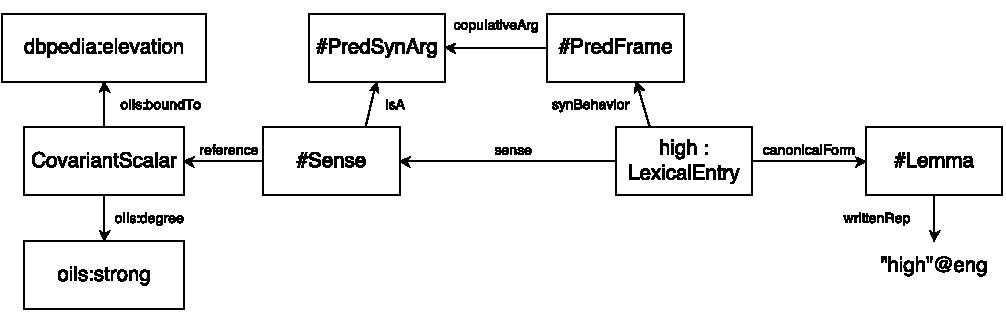
\includegraphics[width=\textwidth]{high-example}
\caption{An example of the modelling of `high' in \emph{lemon}\label{high-example}}
\end{figure}

\begin{verbatim}
high: a lemon:LexicalEntry ;
  lemon:canonicalForm high:Lemma ;
  lemon:synBehavior high:PredFrame ;
  lemon:sense high:Sense .

high:Lemma lemon:writtenRep "high"@eng .

high:PredFrame lexinfo:copulativeArg high:PredArg .

high:Sense lemon:reference [
    rdfs:subClassOf oils:CovariantScalar ;
    oils:boundTo dbpedia:elevation ;
    oils:degree oils:strong ] ;
  lemon:isA high:PredArg .
\end{verbatim}

\textbf{Thresholds and multiple classes}

Finally, we turn to the case of operator adjectives, where we will not be able to easily create a vocabulary that can fully describe the semantics of the adjective within the context of OWL as the second nature order of the logic cannot be captured well within the framework of description logic. However, for many operator adjectives we can capture the semantics through the \emph{punning} method as described above. To this extent we can understand such adjectives as object properties, whose value is a punned class. To do this we need to add a frame on the syntax side, that indicates that the argument of the adjective is in fact the noun phrase. We would do this as follows (figure \ref{former-example}):

\begin{figure}
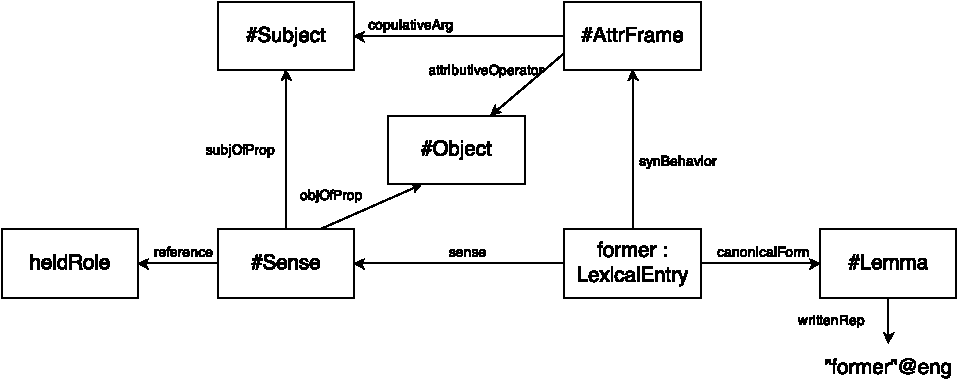
\includegraphics[width=\textwidth]{former-example}
\caption{An example of modelling `former' in \emph{lemon}\label{former-example}}
\end{figure}

\begin{verbatim}
former: a lemon:LexicalEntry ;
	lemon:canonicalForm former:Lemma ;
	lemon:synBehavior former:OperatorFrame ;
	lemon:sense former:Sense .

former:Lemma lemon:writtenRep "former"@eng .

former:OperatorFrame lexinfo:copulativeArg former:Subject ;
  lexinfo:attributiveOperator former:Object .
  
former:Sense lemon:reference onto:heldRole ;
  lemon:subjOfProp former:Subject ;
  lemon:objOfProp former:Object .
\end{verbatim}

The usage of this frame is intended such that a phrase such as

\begin{quote}
Clinton is a former president
\end{quote}

Is interpreted as

\begin{verbatim}
ontology:Clinton ontology:heldRole ontology:President .
\end{verbatim}

\section{Adjectives in question answering}

(Christina, some examples for QALD)

\section{Related work}

The categorization of adjectives in terms of formal semantics goes back to Montague\shortcite{montague1970english}, however one of the most significant attempts to assign a formal meaning was carried out in the Mikrokosmos project\cite{raskin1995lexical}. 


Adjective based inference (Amoia and Gardent)
Adjectives A uniform semantic approach (Abdullah Frost)
Treatment of adjectives in SIMPLE: Theoretical Observations (Peters and Peters)
The Description of Adjectives for Natural Language Processing: Theoretical and Applied Perspectives (Bouillon and Viegas)


\section{Conclusion}

\section*{Acknowledgements}

\bibliographystyle{acl}
\bibliography{cogalex-adjectives}

\end{document}
